\documentclass[12pt,a4paper, xcolor={usenames,dvipsnames,svgnames,table}]{beamer}
\usepackage{presentationStyle}
\usepackage{arydshln,leftidx,mathtools}
\newcommand{\subfigure}{\subfloat}
\renewcommand{\d}{\partial}
%\setbeameroption{show only notes}
\AtBeginSection[]
{
  \begin{frame}
    \frametitle{Outline}
    \tableofcontents[currentsection]
  \end{frame}
}
%\AtBeginSubsection[]
%{
%  \begin{frame}
%    \frametitle{Outline}
%    \tableofcontents[currentsection,currentsubsection]
%  \end{frame}
%}
\setbeamertemplate{section in toc}[ball unnumbered]
\title % (optional, only for long titles)
{Multiscale modeling of diffusion processes in dendrites and dendritic spines}
%\subtitle{Evidence from India}
\author % (optional, for multiple authors)
{Fredrik Eksaa Pettersen\inst{1}}
\institute[UiO] % (optional)
{
  \inst{1}%
  Faculty of Mathematics and Natural Sciences\\
  University of Oslo
}
\date% (optional)
{June $26^{\text{th}}$, 2014}
\subject{Master thesis presentation}
\begin{document}

% ------- TITLE -------- %
\frame[plain]{\titlepage}
\notetoself{Welcome. Today, I will be presenting my masters thesis, \textbf{Multiscale modeling of diffusion processes in dendrites and dendritic spines.}}


% ------ OUTLINE --------%
\begin{frame}{Outline}
\tableofcontents
%\frametitle{Testing}
%\begin{itemize}
%\pause \item Medical background
%\pause \item The simulation scenario
%\pause \item Mathematical models
%\pause \item Discretization
%\pause \item Implementation
%\pause \item Results
%	\begin{itemize}
%	\item Verification of implementation
%	\item Simulation results
%	\end{itemize}
%\pause \item Conclusions
%\end{itemize}
\end{frame}
\notetoself{Here is an overview of the presentation. I will begin by giving a motivation for developing a multi scale solver before I move on to describe some of the theory that is necessary. Next, I will describe some very useful test that the code must pass in order to verify that it is implemented correctly, and describe an application that illustrates how the software can be modified to describe physical problems. Finally, the results of the verification and application will be discussed and some concluding remarks will be given.}


% ----- INTRODUCTION ----- %
\section{Motivation}
\note{I will start of by motivating the need for a hybrid diffusion solver.}
%\addcontentsline{toc}{section}{ -- Medical background}

\subsection{Physical models on different length scales}
\begin{frame}[shrink]
\frametitle{Physical models on different length scales}
\begin{columns}
 \column{0.5\textwidth}
\begin{itemize}
\item<2-> Systems on different length scales are characterized by different effects.
\item<3-> Quantum Mechanics is the ``typical'' example in physics, but there are many more.
\item<4-> Problems might arise between these length scales
\end{itemize}
 \column{0.5\textwidth}
\begin{figure}[H]
  \centering
  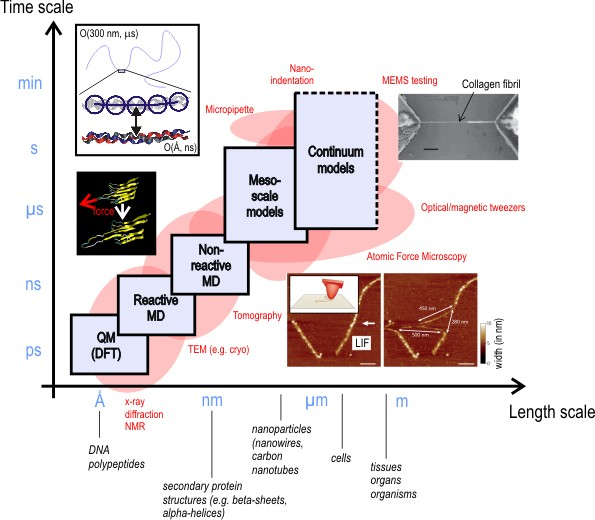
\includegraphics[width=\textwidth]{Figures/lengthscales.jpg}
  \caption{Illustration of physical models on different length scales, from  Markus J. Buehler, MIT}
 \end{figure}
\end{columns}
\end{frame}
\notetoself{}


\begin{frame}[shrink]
\frametitle{Physical models on different length scales}
\framesubtitle{Existing meso scale models}
Some meso scale models exist already, but mostly these are aimed at specific problems and/or closed source.
\begin{itemize}
 \item Dissipative Particle Dynamics
 \item Dendritc solidification modeling by 
 \item Hybrid fluid flow models by 
\end{itemize}
\end{frame}
\note{The symptoms of the Chiari I malformation are very diverse, making the condition difficult to diagnose without the use of magnetic resonance imaging. The Chiari I malformation is also related to other conditions, most notably syringomyelia.}

\subsection{Aim of this project}
\begin{frame}
\frametitle{Aim of this project}
\begin{itemize}
\item<2-> Develop and implement a hybrid diffusion solver using Random Walk as a lower scale model.
\item<3-> Make sure all parts of the theory are transparent.
\item<4-> Test and verify implementation thoroughly.
\item<5-> Apply developed software to physical problem in order to verify functionality.
\end{itemize}
\end{frame}
\note{Syringomyelia is a condition in which fluid-filled cavities, also known as sytinxes, develop in the spinal cord tissue. Syrinxes may cause irreversible nerve damage; however, the reason why syrinxes form is yet to be determined. Estimated It is estimated that approximately $70\%$ of syringomyelia is related to hindbrain malformations such as the Chiari I malformation, and approximately $30-50\%$ of Chiari patients develop syrinxes. This thesis investigated the response of the spinal cord under pressure caused by CSF flow, to see if a mathematical model for the spinal cord could further understanding of syrinx formation.}

%\subsection{CSF flow}
%\begin{frame}
%\frametitle{CSF flow}
%Cerebrospinal fluid (CSF) flows in the subarachnoid space (SAS) in the brain and spinal column.
%\begin{itemize}
%\item<1-> Studies show that Chiari I results in abnormal CSF flow.
%\begin{itemize}
%\item<2-> Velocity
%\item<2-> Pressure
%\end{itemize}
%\item<2-> Believed to be a possible cause for symptoms and syringomyelia.
%\end{itemize}
%\end{frame}


\section{Theory}
%\addcontentsline{toc}{section}{ -- Simulation scenario}
\notetoself{We now continue to the simulation scenario. To understand what exactly is to be simulated, the spinal cord is studied.}


%\subsection{Spinal cord}
%\begin{frame}
%\frametitle{The spinal cord}
%\begin{multicols}{2}
%\begin{itemize}
%\item<2-> Part of the central nervous system.
%\item<3-> Encased in the spinal column.
%\item<4-> CSF flows past the spinal cord.
%\item<5-> Cylindrical in shape.
%\item<6-> Made up of grey and white matter.
%\end{itemize}
%\vspace{2cm}
%\begin{figure}
%\centering
%\includegraphics[width=0.55\textwidth]{\imagepath/vertebra-cross-section.jpg}
%\end{figure}
%\end{multicols}
%\end{frame}
%\notetoself{The spinal cord, together with the brain, makes up the central nervous system. It is located within the spinal column, and protected by three layers of membranes known as the pia mater, arachnoid and dura mater. Between the pia and arachnoid is the subarachnoid space (SAS), in which CSF flows. It is from this flow that pressure is applied on the spinal cord. The spinal cord is cylindrical in shape, and is made up of a core of grey matter, covered by white matter.}


% ----- SIMULATION SCENARIO ----- %
\begin{frame}{Random Walks}
\begin{multicols}{2}
\begin{itemize}
\item<2-> Widely used in many applications.
\item<3-> Can be shown to fulfill the diffusion equation.
\item<4-> Used as lower scale model for this purpose
\end{itemize}
\begin{figure}
\centering
\includegraphics[width=0.5\textwidth]{Figures/randomwalk.eps}
\end{figure}
\end{multicols}
\end{frame}
\notetoself{In the simulations, an anatomically accurate geometry is used to represent the spinal cord. This geometry is based on the spinal cord of a sheep, and is approximately 3.4 cm in length. }


\begin{frame}{Finite difference methods}
\framesubtitle{- For partial differential equations}
\begin{columns}
 \column{0.5\textwidth}
\begin{itemize}
\item<2-> Approximate derivatives by finite differences using the definition of the derivative and omitting the limit:
\begin{align*} 
 \frac{du}{dt} &=\lim_{\Delta t\to0} \frac{u(t) -u(t+\Delta t)}{\Delta t} \\
 &\approx \frac{u(t) -u(t+\Delta t)}{\Delta t}
\end{align*}
\item<3-> Repeat for all derivatives in the PDE.
\item<4-> Solve equation on discrete mesh points.
\end{itemize}

\column{0.5\textwidth}
\begin{figure}
\centering
\includegraphics[width=0.5\textwidth]{Figures/FDM_stencils.eps}
\end{figure}
\end{columns}
\end{frame}
\note{To simulate the pressure from CSF flow, measured pressure values from a Chiari patient was used. The pressure was modelled as a travelling wave on the form seen here, where $z$ is the longitudinal coordinate and $c$ is the wave speed, measured to be $2$m/s.}

\begin{frame}{Finite difference methods}
% \framesubtitle{}

\begin{itemize}
\item<2->The two discretizations used are summarized in the theta-rule description 
\begin{equation}
 \frac{u^{k+1}-u^k}{\Delta t} = \theta D\frac{\d^2 u^{k+1}}{\d x^2} + (1-\theta)D\frac{\d^2 u^{k}}{\d x^2}.
\end{equation}
\item<3->In order to accommodate a larger time step, the Backward Euler discretization ($\theta =1$) must be implemented:
{\footnotesize
\begin{align*}
 u^{k+1}_i = \frac{D\Delta t}{\Delta x^2}\left((u^{k+1}_{i+1}-u^{k+1}_{i})-(u^{k+1}_{i}-u^{k+1}_{i-1})\right) + u^k_i.
\end{align*}
}
\item<4-> By insertion the BE scheme results in a tridiagonal linear system in 1D.
\end{itemize}
\end{frame}


\begin{frame}{Tridiagonal linear systems}
 Tridiagonal linear systems are efficiently solved by a specialized Gaussian elimination algorithm.
 {\footnotesize
 \lstinputlisting[label=theory:tridiag,caption=The tridiag algoritm,language=c++]{../Figures/tridiag2.cpp}
 }
\end{frame}


\begin{frame}{Finite difference methods}
\framesubtitle{Backward Euler in 2D}

\begin{itemize}
\item<2-> In 2D the solution to the discrete diffusion equation is a matrix.
\item<3-> Rewriting the matrix as a vector results in a banded linear system:
{\footnotesize
\begin{align*}\label{linear_system_BE2D}
  \left(\begin{array}{c c c : c c c : c c c}
        \gamma & -2\beta &0 &-2\alpha &0 &0 &0 &0 &0\\
        -\beta & \gamma & -\beta &0 &-2\alpha &0 &0 &0 &0\\
        0&-2\beta & \gamma & 0 & 0 & -2\alpha &0&0&0\\ \hdashline
        -\alpha& 0&0 & \gamma & -2\beta & 0 & -\alpha &0&0\\
        0& -\alpha&0&-\beta & \gamma & -\beta & 0 & -\alpha &0\\
        0& 0& -\alpha&0&-2\beta & \gamma & 0 & 0 &-\alpha\\ \hdashline
        0& 0 &0 &-2\alpha &0&0 & \gamma & -2\beta&0\\
        0& 0 &0 &0 &-2\alpha&0&-\beta & \gamma &-\beta\\
         0&0 &0 &0&0 &-2\alpha&0&-2\beta & \gamma
       \end{array}\right)\mathbf{u} = \mathbf{u}_p
\end{align*}
}
\end{itemize}
\end{frame}

\begin{frame}{Tridiagonal linear systems}
 \framesubtitle{Block tridiagonal solver}
The tridiag algorithm can be rewritten to solve block tridiagonal systems by replacing divisions with matrix inverses:
\begin{align*}
 H_0 &= -B_0^{-1}C_0\nonumber \\
 \mathbf{g}_0 &= B_0^{-1}\mathbf{u}_{p0} \nonumber\\
 H_i &= -\left(B_i+A_iH_{i-1}\right)^{-1}C_i \nonumber \\
 \mathbf{g}_i &= \left(B_i+A_iH_{i-1}\right)^{-1}\left(\mathbf{u}_{pi}-A_i\mathbf{g}_{i-1}\right)\\
 \text{}\\
  \mathbf{u}_{n-1} &= \mathbf{g}_{n-1}\nonumber\\
  \mathbf{u}_i &= \mathbf{g}_i + H_i\mathbf{u}_{i+1} \nonumber
 \end{align*}
\end{frame}

\begin{frame}{Tridiagonal linear systems}
 \framesubtitle{Performance of Block tridiagonal solver}
 \begin{itemize}
  \item <1-> The 1D tridiagonal solver requires $\mathcal{O}(n)$ operations, comparable to the Forward Euler scheme.
  \item <2-> The Block tridiagonal solver requires inversion of $2n$ matrices, but only once.
  \item <3-> In total $\mathcal{O}(n^{2d-1})$ operations are required for a general system, one order less than e.g. LU decomposition.
  \item <4-> Memory impact can also be reduced to $8\cdot n^{2d-1}$ bytes, as opposed to $8\cdot n^{2d}$ bytes.
 \end{itemize}
\end{frame}

\section{Details of the coupling}
\notetoself{In order to simulate the response of the spinal cord under applied pressure, mathematical models for the spinal cord are needed. The spinal cord is considered a solid. Because the spinal cord has been shown to display viscoelastic properties, a viscoelastic model is used. In addition, a purely elastic model is used for comparison.}
%\addcontentsline{toc}{section}{ -- Mathematical models}
% ----- MATHEMATICAL MODELS ----- %

\subsection{The algorithm}
\begin{frame}[shrink]{The algorithm}
After the initial setup, the algorithm is as follows:
\begin{itemize}
 \item<2-> The result from previous PDE time step, $\mathbf{u}_p$, is converted to a distribution of random walkers and sent to the RW solver.
 \item<3-> The RW solver does a predefined number of micro scale time steps which correspond to one PDE time step.
 \item<4-> The result from the RW solver is converted back to a concentration and this replaces the PDE solution, $\mathbf{u}_p$.
 \item<5-> $\mathbf{u}_p$ is then used as input to calculate the next time step.
\end{itemize}

\end{frame}
\notetoself{\small The governing equations from the theory of elasticity are given here. Gamma D denotes the Dirichlet boundary and Gamma N denotes the Neumann boundary. The Neumann boundary condition simulated the applied pressure, where p is the travelling wave from the previous slide. The Dirichlet boundary condition is used to place constraints on the solution, and in this particular case the Dirichlet boundary was chosen to be the top and bottom boundaries, where the geometry would be connected to more spinal cord above and below. There are no obvious choices for what this condition should be. $u=0$ is a possibility, although that would not allow the spinal cord to compress in the radial direction at the boundaries. }
\note{Another possibility is $u_z=0$. Dirichlet boundary conditions will be discussed in more detail later, and for now we leave $u=u_D$.}

\begin{frame}
\frametitle{Conversion between length scales}
\begin{columns}
 \column{0.5\textwidth}
\begin{itemize}
\item<2-> A single, real integer converts the concentration in one mesh point to a number of random walkers.
\item<3-> \begin{equation*}
            C_{ij} = Hc\cdot u_{ij}
          \end{equation*}
\item<4-> The conversion must be done at each time step because the concentration over an area of the mesh might change.
\end{itemize}
 \column{0.5\textwidth}
 \begin{figure}[H]
  \centering
\includegraphics[width=\textwidth]{../Figures/integral_illustration.eps}
  \end{figure}

\end{columns}
\end{frame}

\subsection{Coupling the models through the step length}
\begin{frame}
\frametitle{Coupling the models through the step length}
\begin{itemize}
 \item<1-> The RW solver needs a constraint in order to make sure it models diffusion on the same time scale as the PDE model.
 \item<2-> From an Einstein relation we find
 \begin{equation*}
  \langle\tilde{\Delta x}^2\rangle = 2Dd\tilde{\Delta t}
 \end{equation*}
 \item <4-> Rewriting this results in the desired restriction which is placed on the step length:
 \begin{equation*}
 l = \sqrt{2dD\frac{\Delta t}{\tau}}
\end{equation*}
\end{itemize}

\end{frame}
\notetoself{In order to describe the specific behavior of a material, a constitutive relationship is required. In particular, we want a stress-strain relationship. Sigma, as appears in the governing equations, is the stress tensor, while the strain tensor is defined as shown. The constitutive relationships we are looking for is then the stress expressed in terms of the strain.  For simplicity, only linear constitutive relationships have been considered, for isotropic materials.}

\subsection{Boundary Conditions}
\begin{frame}
\frametitle{Boundary conditions on the random walk}
\begin{itemize}
 \item<1-> Perfectly reflecting boundaries, equivalent to zero flux
 \begin{equation*}
   \frac{\d C}{\d n} = 0
 \end{equation*}
 \item<2-> Updating concentration at each time step must also be considered a boundary condition.
 \item<3-> Other boundary conditions might have been better, say perfect flux exchange:
 \begin{equation*}
   \frac{\d u}{\d n} = \frac{\d C}{\d n}
 \end{equation*}
 \item<4-> Requires some work on the PDE boundary conditions etc.
\end{itemize}

\end{frame}
\notetoself{}



\section{Verification}
\notetoself{With the mathematical models in place, they may be discretized in order to be implemented on a computer.}
% ------ DISCRETIZATION ------ %
\subsection{Error estimate}
\begin{frame}{Computation of the error}
\begin{itemize}
 \item<1-> Solving PDEs by FDMs results in errors which can tell a lot about the implementation.
 \item<2-> From the residuals, we know how the error should behave.
 \item<3-> For a given exact solution, $u_e$, the error is defined by:
 \begin{align*}
  \epsilon(t^k) &= ||u(t^k)-u_e(t^k)||_2 \\
   &\approx \sqrt{\Delta x\Delta y\sum\limits_{i=0}^k\sum\limits_{i=0}^k \left(u(t^k,x_i,y_j)-u_e(t^k,x_i,y_j)\right)^2}.
 \end{align*}

\end{itemize}
\end{frame}
\notetoself{}


\subsection{Verification techniques}

\begin{frame}[shrink]
\frametitle{Verification techniques}
\framesubtitle{Method of manufactured solutions}
\begin{itemize}
 \item<1-> Make a solution by adapting the source term.
 \item<2-> For example:
 \begin{align*}
  u(x,t) = \frac{1}{x+1}\\
  \implies s(x,t) = \frac{2D}{(x+1)^3}
 \end{align*}
 \item<3-> Many useful variations of this method.
 \item<4-> Tests are done using 
  \begin{equation*}
  u(x,y,t) = e^{-\pi^2t}\cos(\pi x)\cos(\pi y) +1,
 \end{equation*}
 which fulfills boundary conditions and has $s(x,t) = 0$.
\end{itemize}
\end{frame}
\notetoself{}


\begin{frame}[shrink]
\frametitle{Verification techniques}
\framesubtitle{Convergence tests}
\begin{itemize}
 \item<1-> Error term is on the form
 \begin{equation*}
 \epsilon = C_x\Delta x^2 + C_t\Delta t^1,
\end{equation*}
for the schemes that are implemented.
\item<2-> Measuring the exponents gives the convergence of the scheme.
\item<3-> Do several simulations and calculate
\begin{equation*}
 r\simeq \frac{\log\left(\epsilon_1/\epsilon_2\right)}{\log\left(\Delta t_1/\Delta t_2\right)}.
\end{equation*}
\item<4-> Often difficult tests.
\end{itemize}
\end{frame}
\notetoself{}

\begin{frame}[shrink]
\frametitle{Verification techniques}
\framesubtitle{Numerical exact solutions}
\begin{itemize}
 \item <1-> Discretization is a reformulation of a PDE as a difference equation. 
 \item <2-> New exact solution can be found - theoretically zero error!
 \item <3-> Forward Euler solution (1D):
 \begin{equation*}
  u^{k+1} = \sum\limits_{i=0}^k {k\choose i}\left(D\Delta t\right)^i\frac{2^i}{\Delta x^{2i}}\left(\cos(\pi\Delta x)-1\right)^i\cos(\pi x).
 \end{equation*}
 \item <3-> Backward Euler solution:
 \begin{equation*}
   \vec u^{k} = \left(\mathbf M^{-1}\right)^{k} \vec u^0.
 \end{equation*}
\end{itemize}
\end{frame}



\section{Application}
\notetoself{Now that the boundary conditions are dealt with, the problem may be implemented.}
% ------ IMPLEMENTATION ------ %
\begin{frame}[shrink]{The problem}
\begin{columns}
\column{0.5\textwidth}
\begin{itemize}
 \item <2-> Pyramidal neuron
 \item <3-> Protein Kinase C$\gamma$
 \item <4-> Dendritic spines
\end{itemize}

\column{0.5\textwidth}
\begin{figure}[H]
 \centering
 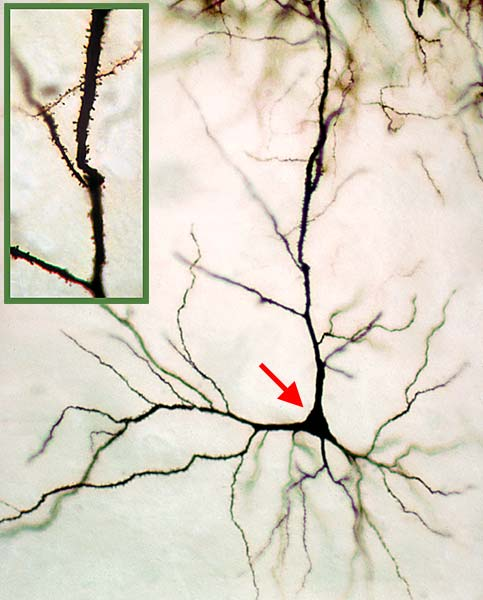
\includegraphics[width=\textwidth]{../Figures/Cochlear_nucleus_multipolar_cell.jpg}
\end{figure}

\end{columns}

\end{frame}
\notetoself{}


\begin{frame}[shrink]{Computational model}

\begin{columns}
\column{0.5\textwidth}
Default setup
\begin{figure}[H]
 \centering
 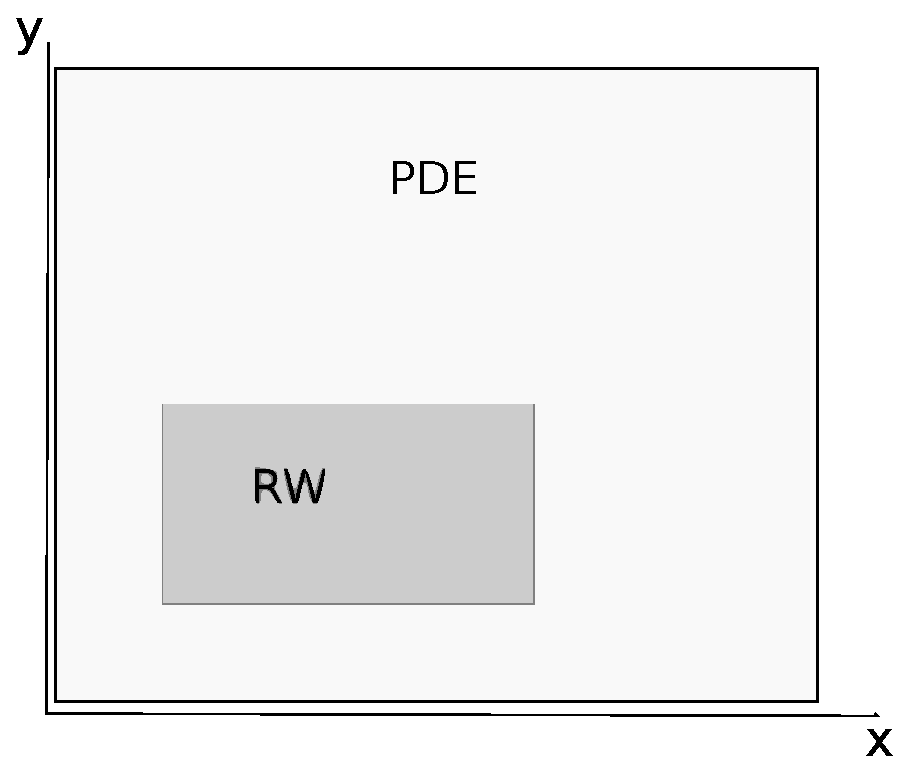
\includegraphics[width=\textwidth]{../Figures/hybrid_model_principle.eps}
\end{figure}
\column{0.5\textwidth}
Modified setup
\begin{figure}[H]
 \centering
 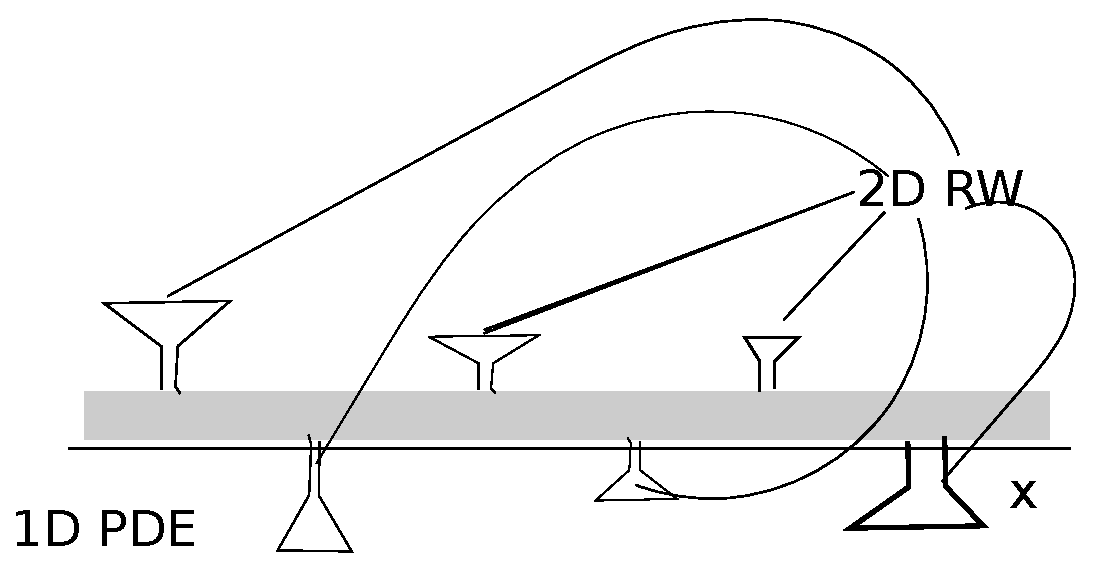
\includegraphics[width=\textwidth]{../Figures/dendrite_spine_model.eps}
\end{figure}
\end{columns}
\end{frame}
\notetoself{}


\begin{frame}[shrink]{Parameters and other details}
\begin{itemize}
 \item <1-> Craske et.al. report increases of 5$\frac{\text{nMol}}{\text{L}}$ in spines.
 \item <2-> Corresponds to 1-2 walkers, using values from Arellano et.al.
 \item <3-> Spine geometries chosen at random to correspond with Arellano et.al.
 \item <4-> Initial condition is modified to accommodate absorption effects (\url{http://jcb.rupress.org/content/170/7/1147/suppl/DC1}).
\end{itemize}
\end{frame}
\notetoself{}

\section{Results}
\notetoself{This brings us to the simulations. Results from the simulations will now be reviewed.}
% ------ RESULTS ------ %
\subsection{Results of verification}
\begin{frame}[shrink]{What we are looking for}
\begin{itemize}
 \item Successful tests of PDE solvers.
 \item Successful tests of RW solver.
 \item Successful test of hybrid solver given sufficient number of walkers.
\end{itemize}

\end{frame}
\notetoself{}


\begin{frame}[shrink]{PDE solvers}
% Include one Convergence test, and numerical exact solution plot for each scheme!
\begin{columns}
 \column{0.5\textwidth}
\vspace{5pt}\\ BE
 \begin{figure}[h!]
 \centering
  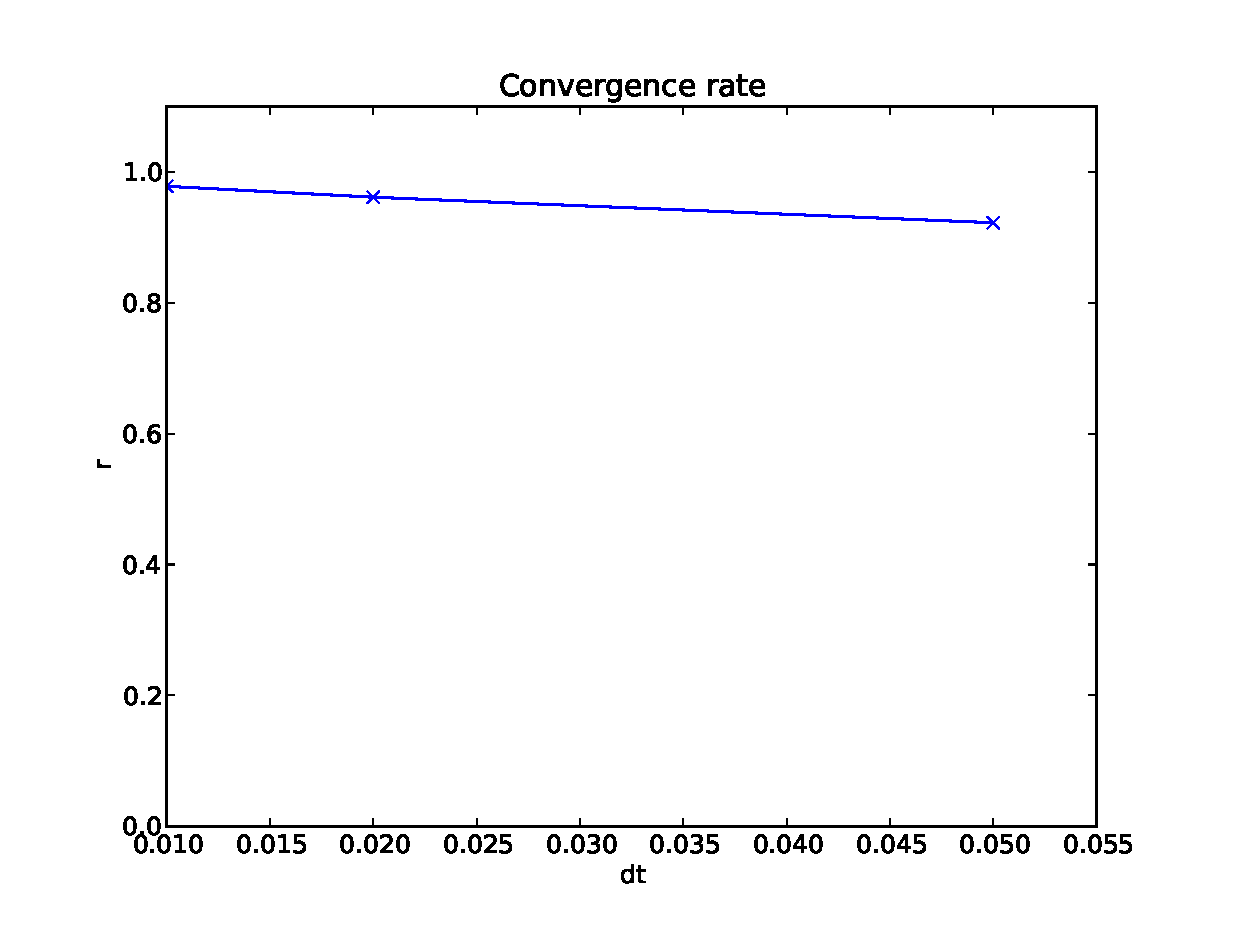
\includegraphics[width=0.8\textwidth]{../../results/experiment_14052014_0744_errorplot_BE1D/results/ConvergenceTest.eps}
 \end{figure}
 \begin{figure}[h!]
 \centering
  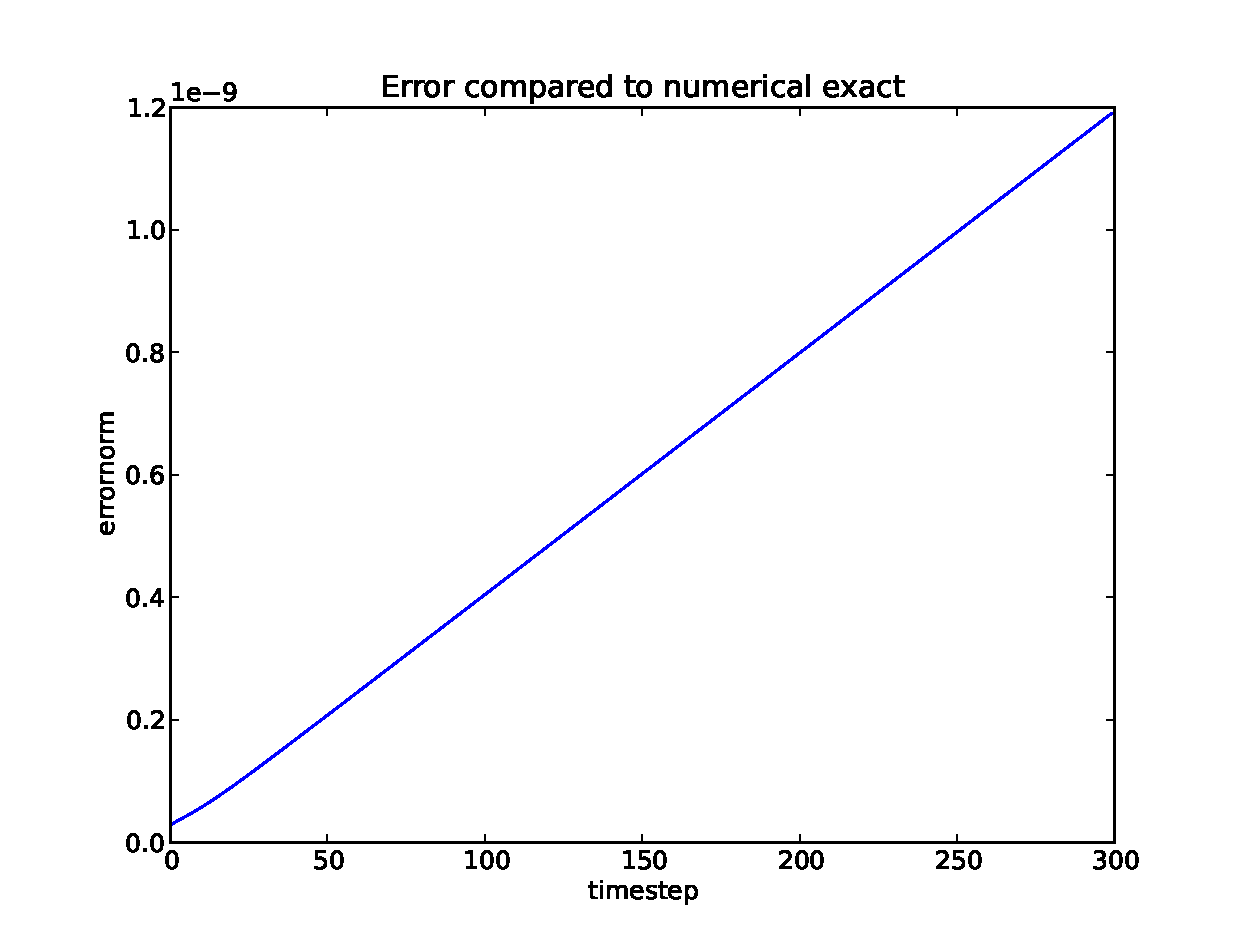
\includegraphics[width=0.8\textwidth]{../../results/experiment_14042014_0759_BE1D_numerical_exact/results/numerical_exact.eps}
%  \end{subfigure}
 \end{figure}

\column{0.5\textwidth}
\vspace{5pt} \\FE
 \begin{figure}[h!]
 \centering
  \includegraphics[width=0.8\textwidth]{../../results/experiment_27052014_1152_FE2D_new_convergence_time/results/ConvergenceTest_pretty.eps}
 \end{figure}
 \begin{figure}[h!]
 \centering
  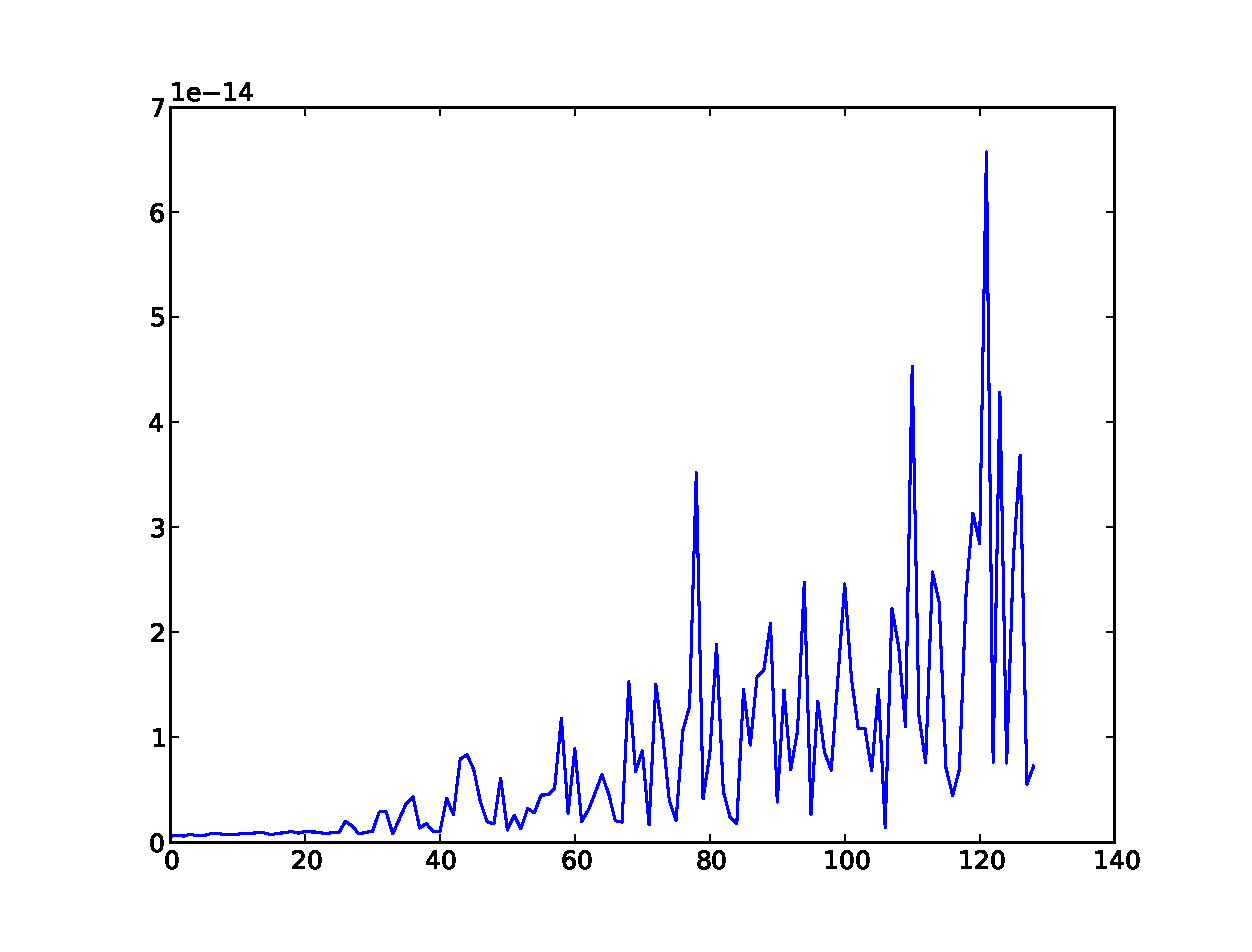
\includegraphics[width=0.8\textwidth]{../Figures/exact_numerical_1d_n130.eps}
 \end{figure}
\end{columns}

\end{frame}
\notetoself{}


\begin{frame}[shrink]{RW solver}
\begin{columns}
 \column{0.5\textwidth}
 \begin{itemize}
  \item <2-> Needs a new initial condition, otherwise similar.
  \item <3-> No numerical exact solution.
  \item <4-> Expected convergence rate of $0.5$.
  \item <5-> Verifies that the coupling works.
 \end{itemize}
\column{0.5\textwidth}
\vspace{5pt}\\
\begin{figure}[H]
 \centering
  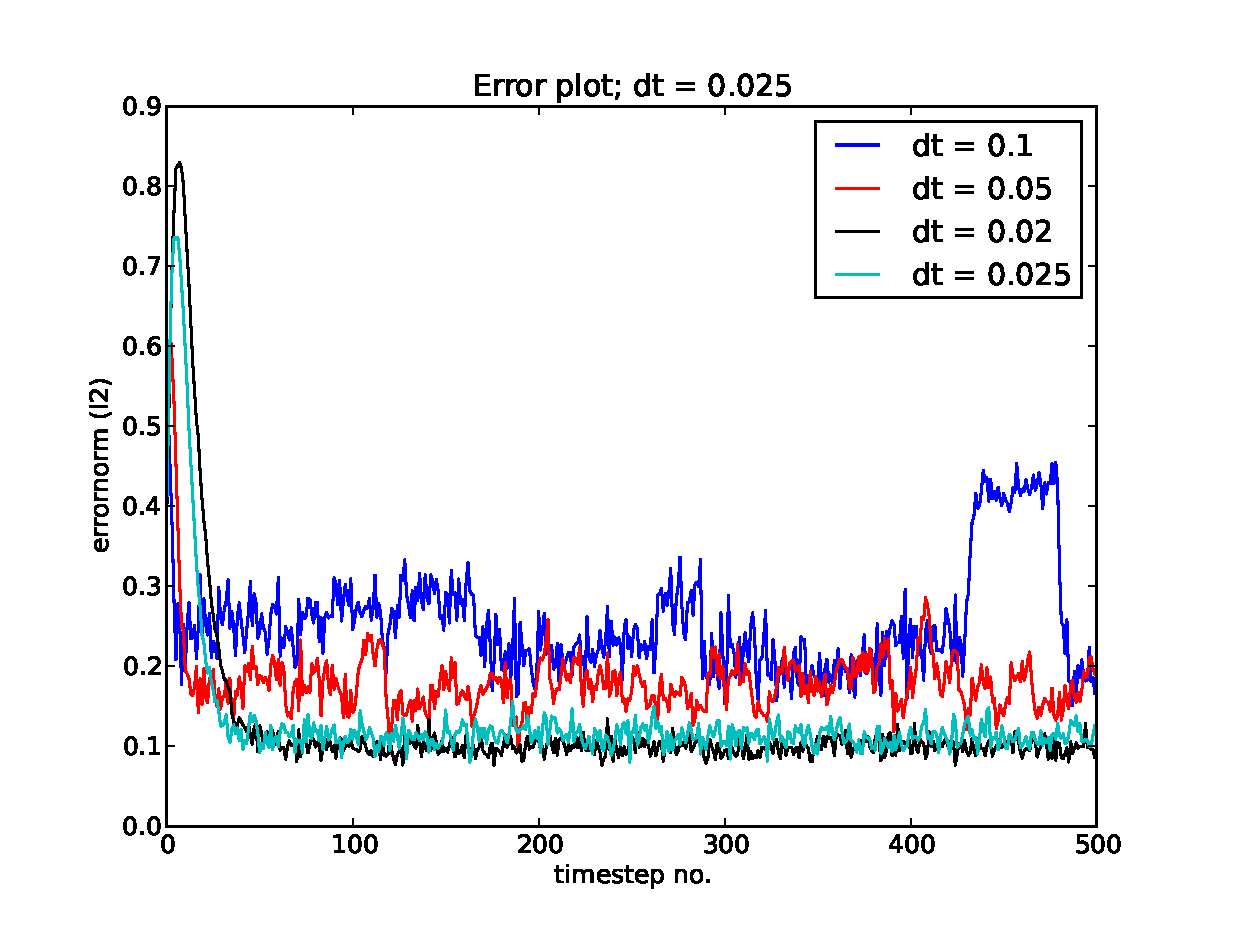
\includegraphics[width=0.8\textwidth]{../../results/experiment_01052014_1615_Redoing_RW_tests/results/errorplot.eps}
\end{figure}
\begin{figure}[h!]
\centering
  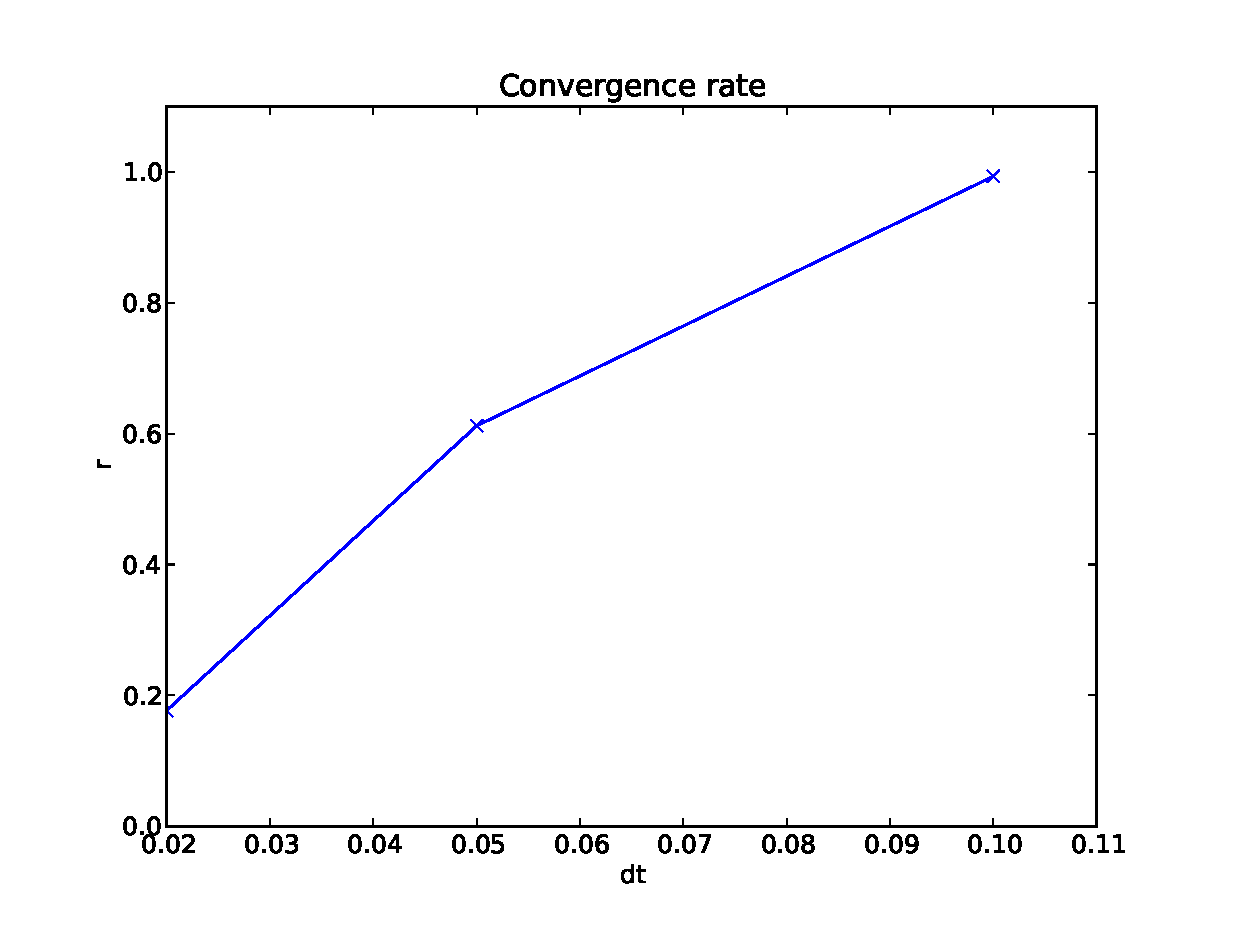
\includegraphics[width=0.8\textwidth]{../../results/experiment_01052014_1615_Redoing_RW_tests/results/ConvergenceTest.eps}
\end{figure}
\end{columns}

\end{frame}
\notetoself{}


\begin{frame}[shrink]{Hybrid solver}
\begin{columns}
 \column{0.5\textwidth}
 \vspace{5pt}\\
 \begin{itemize}
 \item <2-> New error term:
 \begin{equation*}
   \epsilon(t) = C_t \Delta t + C_x \Delta x^2 + \frac{C_{RW}}{\sqrt{Hc}}
 \end{equation*}
 \item <2-> A lot of walkers are required:
 \begin{equation*}
  Hc \geq \frac{1}{\Delta t^2}
 \end{equation*}
  \item <3-> Expect first order convergence.
  \item <4-> The extra error can be controlled (at a large cost).
 \end{itemize}
\column{0.5\textwidth}
\vspace{5pt}\\
\begin{figure}[H]
 \centering
  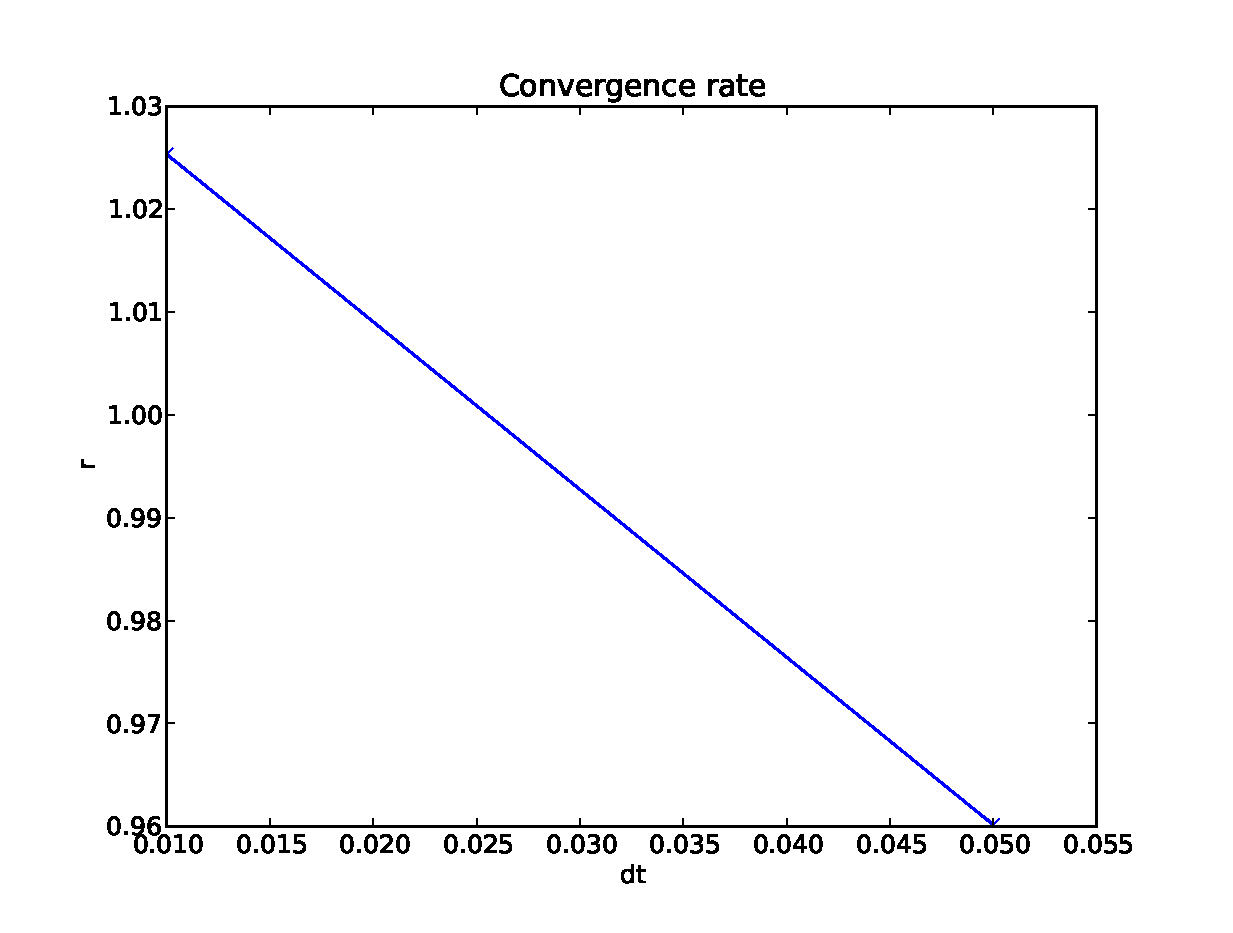
\includegraphics[width=\textwidth]{../../results/experiment_15042014_0608_convergence_tests_etc/results/ConvergenceTest.eps}
\end{figure}
\end{columns}
\end{frame}
\notetoself{}

\subsection{Application}
\begin{frame}[shrink]{Results from application}
\begin{columns}
 \column{0.5\textwidth}
 \begin{itemize}
  \item <2-> Consistently towards lower range of results by Craske et.al.
  \item <3-> Otherwise relatively good.
  \item <4-> $\sim$ 2-3 seconds can be added.
 \end{itemize}
 \column{0.5\textwidth}
 \begin{figure}[H]
  \centering
  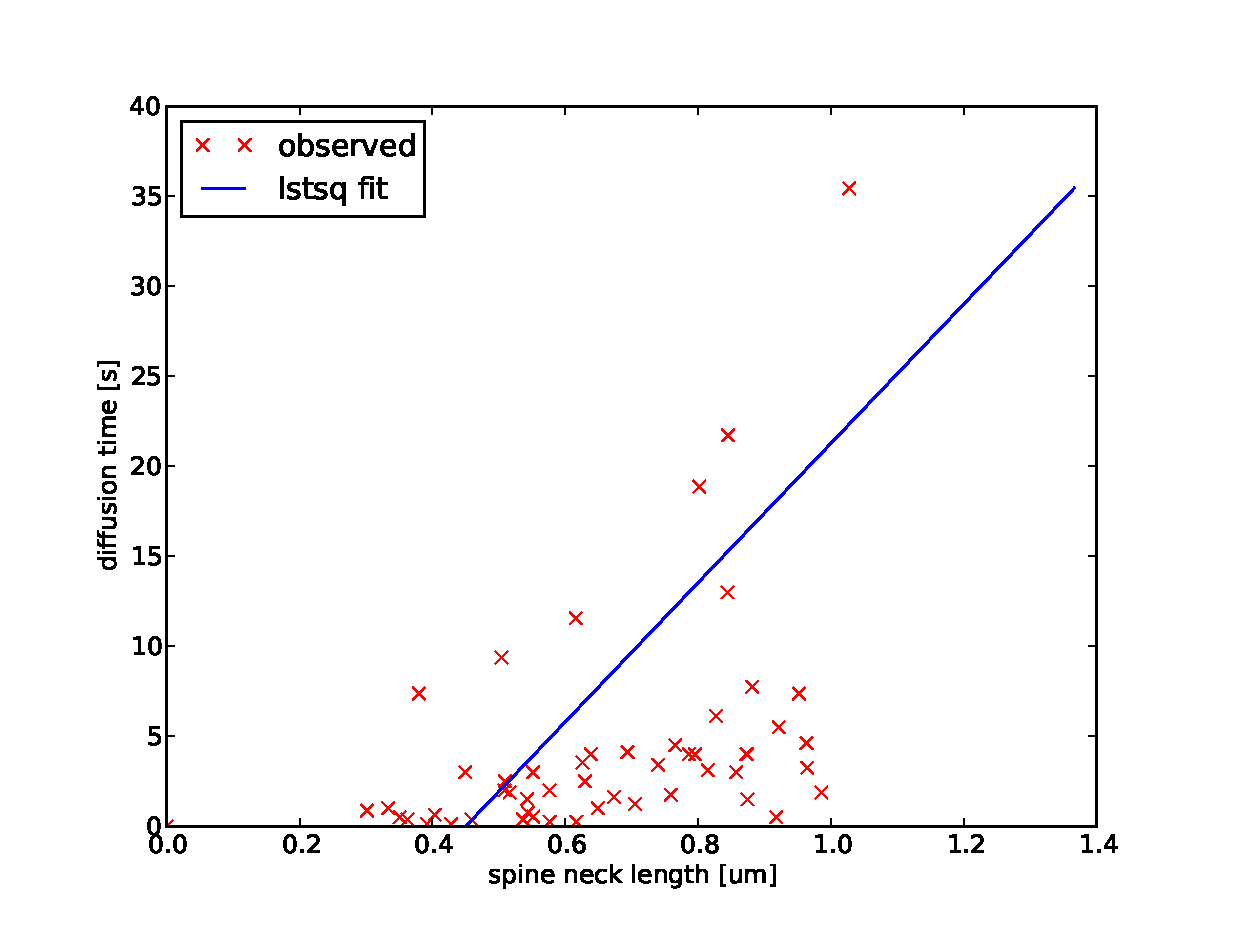
\includegraphics[width=0.9\textwidth]{../Figures/spine_stats_reltime_nl.eps}
 \end{figure}
 \begin{figure}[H]
  \centering
  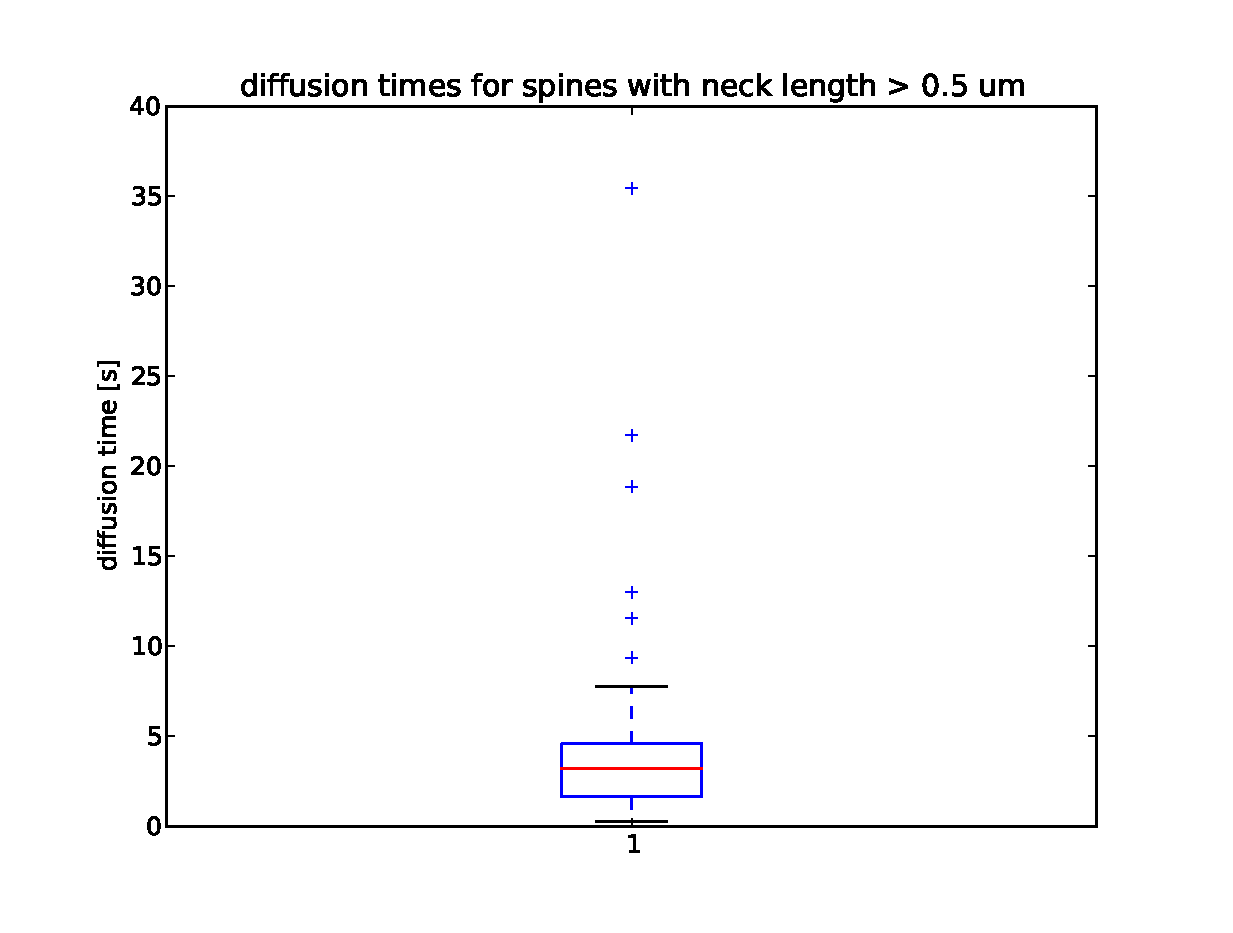
\includegraphics[width=0.9\textwidth]{../Figures/spine_stats_boxplot_reltime_longneck.eps}
 \end{figure}
\end{columns}

\end{frame}
\notetoself{}



\section{Concluding remarks}
\subsection{Conclusions}
\notetoself{The simulation results and verification tests allow some conclusions to be made. Some suggestions for further work are also provided.}
% ------ CONCLUSIONS ------ %
\begin{frame}[shrink]{Conclusions}
\begin{itemize}
\item<2-> Both PDE, RW and hybrid solvers are implemented correctly.
\item<3-> Software can be modified to model real applications.
\item<4-> Proof of concept.
\end{itemize}
\end{frame} 
\notetoself{}

\subsection{Further work}
\begin{frame}[shrink]{Further work}
\begin{itemize}
\item<2-> Implement flux exchange boundary conditions
\item<3-> Find other physical applications - anisotropy.
\item<4-> Implement Finite element PDE solver.
\end{itemize}
\end{frame}
\notetoself{}


\begin{frame}[plain]
Thank you for your attention!
\end{frame}


\begin{frame}[allowframebreaks]
  \frametitle<presentation>{References}    
  \begin{thebibliography}{10}    
  %\beamertemplatebookbibitems
  \beamertemplatearticlebibitems
  \bibitem{chiariSymptoms2004}
    {Diane M. Mueller}, ND RN and {John J. Oro'}, MD.
    \newblock {\em Prospective Analysis of Presenting Symptoms Among 265 Patients With Radiographic Evidence of Chiari Malformation Type I With or Without Syringomyelia}.
    \newblock {Journal of the American Academy of Nurse Practitioners}, 16(3), 2004.
  \bibitem{stoverudPia2014}
  St{\o}verud, Karen H. and Aln{\ae}s, Martin and Langtangen, Hans Petter and Haughton, Victor and Mardal, Kent-Andr{\'e}.
  	\newblock{Effect of pia mater, central canal, and geometry on wave propagation and fluid movement in the cervical spinal cord.}
  	\newblock{Manuscript submitted for publication}, 2014.
%  \bibitem{Jemand2000}
%    S.~Jemand.
%    \newblock On this and that.
%    \newblock {\em Journal of This and That}, 2(1):50--100, 2000.
  \end{thebibliography}
\end{frame}
%@article{chiariSymptoms2004,
%	author = {{Diane M. Mueller}, ND RN and {John J. Oro'}, MD},
%	journal = {Journal of the American Academy of Nurse Practitioners},
%	number = {3},
%	publisher = {American Association of Nurse Practitioners},
%	title = {{Prospective Analysis of Presenting Symptoms Among 265 Patients With Radiographic Evidence of Chiari Malformation Type I With or Without Syringomyelia}},
%	volume = {16},
%	year = {2004}
%}



\end{document}